%
% Copyright 2019 Markus Borg, Lund University
%
% This work is licensed under a Creative Commons Attribution-ShareAlike 4.0 International License.
% See http://creativecommons.org/licenses/by-sa/4.0/
%
% The dodument is based on a LaTeX template developed by Jean-Philippe Eisenbarth
% https://github.com/jpeisenbarth/SRS-Tex
%
\documentclass{scrreprt}
\usepackage{listings}
%\usepackage{underscore}
\usepackage{graphicx}
\usepackage[bookmarks=true]{hyperref}
\usepackage[utf8]{inputenc}
\usepackage[english]{babel}
\hypersetup{
    bookmarks=false,    % show bookmarks bar?
    pdftitle={Lab 0},    % title
    pdfauthor={Markus Borg},                     % author
    pdfsubject={TeX and LaTeX},                        % subject of the document
    pdfkeywords={TeX, LaTeX, graphics, images}, % list of keywords
    colorlinks=true,       % false: boxed links; true: colored links
    linkcolor=blue,       % color of internal links
    citecolor=black,       % color of links to bibliography
    filecolor=black,        % color of file links
    urlcolor=purple,        % color of external links
    linktoc=page            % only page is linked
}%
\def\myversion{1.0 }
\date{}
%\title
\usepackage{hyperref}
\begin{document}

\begin{flushright}
    \rule{16cm}{5pt}\vskip1cm
    \begin{bfseries}
    	\LARGE{ETSA03-ADM-LAB0}\\
    	\vspace{1.5cm}
        \Huge{Lab 0}\\
        \vspace{0.5cm}
        Basic development skills\\
        \vspace{0.5cm}
        required for ETSA03\\
        \vspace{1.5cm}
        \LARGE{Version \myversion}\\
        %\LARGE{Version \myversion approved}\\
        \vspace{1.5cm}
        Prepared by Markus Borg\\
        %\vspace{1.5cm}
        Dept. of Computer Science, Lund University\\
        \vspace{1.5cm}
        \today\\
    \end{bfseries}
\end{flushright}

%\tableofcontents

\chapter*{Revision History}

\begin{center}
    \begin{tabular}{|c|c|c|c|}
        \hline
	    Name & Date & Reason For Changes & Version\\
        \hline
	    Markus Borg & 2019-02-02 & Initial skeleton. & 0.1\\
        \hline
        Markus Borg & 2019-03-01 & Draft of file systems. & 0.2\\
        \hline
        Markus Borg & 2019-03-04 & Draft of command-line interfaces. & 0.3\\
        \hline
        Markus Borg & 2019-03-04 & Added figure of file system tree. & 0.4\\
        \hline
        Markus Borg & 2019-03-04 & Draft of pointers to version control and JUnit. & 0.5\\
        \hline
    \end{tabular}
\end{center}

\chapter{Introduction}
Lab 0 will introduce some core concepts that you will work with extensively throughout this course. This introductory lab has been added to ensure that everyone gets a chance to practice some fundamental development skills -- the students following the course often represent a wide range of backgrounds. Some of you will wonder why it covers elementary concepts, but from experience we know that the content in this pre-lab is not obvious to everyone. You may certainly skip all exercises related to topics you already know well, but be prepared to answer some questions about Lab 0 during the Lab 1 session.

Lab 0 covers the following topics:
\begin{itemize}
 \item Fundamentals of file systems
 \item Command-line interfaces
 \item Version control
 \item Test automation with JUnit
\end{itemize} 

\chapter{Fundamentals of file systems}
A file system is the way in which files are named and where they are placed logically for storage and retrieval, typically on your computer's hard drive. Without a file system, stored information would be practically impossible  to identify and retrieve. A file system can be considered a type of index for all the data stored on your hard drive. With ever-increasing storage space, the organization and accessibility of individual files are becoming more important than ever.

File systems differ between operating systems, such as Microsoft Windows, macOS and Linux-based systems. Different file systems specify different conventions for naming files, e.g., the maximum number of characters in a file name and which characters are valid in the name. Whether or not file names are case sensitive varies as well. File systems also contain metadata about all files, including file size and attributes. 

Digital file systems and files is a metaphor for the paper-based filing systems using the same logic-based method of storing and retrieving documents: files. Microsoft Windows takes the analogy further by also using folders as part of the terminology, equivalent to the general term: directory.

An important feature of a file system is that they introduce a format to specify the path to a file through the structure of directories. Each file is placed in a directory or subdirectory at the desired place in the tree structure, see Figure~\ref{fig:tree}.\\

\begin{figure}
\centering
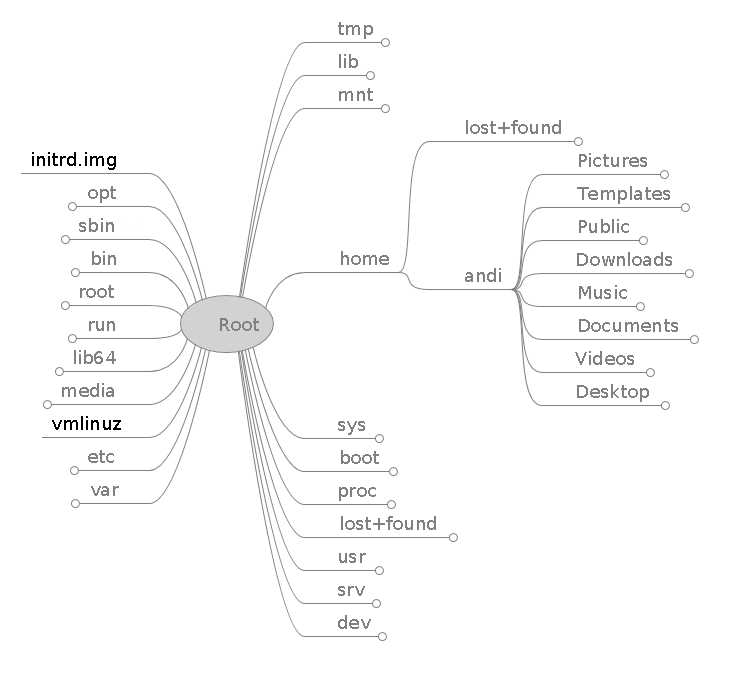
\includegraphics[width=0.5\textwidth]{figures/GNU-Linux_directory_tree.png}
\caption{Part of a GNU/Linux directory tree. (CC BY-SA 3.0, Wikimedia Commons: And1mu).}
\label{fig:tree}
\end{figure}

\textbf{Tasks:} If you have never browsed the file system of your computer, do it now. Identify the default location of downloaded files and where you have stored work in various courses. Where do you plan to install Robocode? Where do you plan to clone the repositories related to the labs and to the project work? 

\chapter{Command-line interfaces}
A command-line interface is a way to interact with a computer program through  commands to the program in the form of successive lines of text, i.e., command lines. A program which handles this interface is referred to as a command language interpreter or shell. Command-line interfaces were the primary means of interaction with most computer systems from the 1960s to the 1980s. Today, most users rarely, if ever, use command-line interfaces and instead rely entirely on graphical user interfaces -- but advanced users often rely on this traditional approach to interaction.

Software engineers must be able to master command-line interfaces. Textual commands allows engineers to perform tasks more efficiently, configure their development environments, or access program features that are not available through graphical user interfaces. Command lines are much more powerful and versatile than the (by design) restricted graphical counterparts! Using command-lines, options to commands can be given in a few characters -- much appreciated by advanced users. Command-lines also allow automation of repetitive tasks through \textit{scripting} sequences of command lines.

Operating systems come with their specific command-line interfaces. The ETSA03 lab sessions will be conducted in rooms equipped with computers running the open source software operating system Ubuntu, a Linux distribution based on Debian. The deafult shell in Ubuntu is called Bash (The Bourne Again SHell). If you plan to use your own Apple MacBook during the course, you will find that the macOS command-line interface \textit{terminal} is a result from its unix heritage -- the fundamental commands presented below will work both for Bash and terminal. If you plan to use a laptop running Microsoft Windows, however, you will need to run slightly different command-lines in its interpreter \textit{Command Prompt}.\\

\textbf{Tasks:} If you have never used the command-line interface before, it is now time to do so. 

\begin{enumerate}
\item \textbf{Start the command-line interface.} 
\begin{itemize}
\item[Ubuntu] Launch the command-line interpretor directly from the GUI.
\item[macOS] Launch Terminal by using Spotlight search, searching for ``terminal''. Add Terminal to your dock as you will open it every time you work with the course.
\item[Windows] Launch Command Prompt by opening the start menu and typing \texttt{cmd}.
\end{itemize}
\item You will find the command-line interpretor in a separate window. It  provides some contextual information of where in the file system you are currently located and possibly who you are. You will find a cursor highlighting where you can input command-lines -- this is referred to as the prompt.
\end{enumerate}

\section{Basic file system navigation}
\begin{enumerate}
\item \textbf{Show your current position} in the file system (useful if you get lost). Input the corresponding command below:
\begin{itemize}
\item[unix] \texttt{pwd} (print working directory) 
\item[Windows] \texttt{cd} (current directory)
\end{itemize}
\item Now \textbf{list every file and directory in your current directory}. Input the following:
\begin{itemize}
\item[unix] \texttt{ls} (list) 
\item[Windows] \texttt{dir}
\end{itemize}
\item Sometimes you need to also \textbf{list the metadata of the files}. Input the command again, but now with an additional option:
\begin{itemize}
\item[unix] \texttt{ls -l}
\item[Windows] \texttt{dir /a}
\end{itemize}
\item You can now continue \textbf{navigating the tree structure of your file system}. Move into a subdirectory by typing:
\begin{itemize}
\item[unix] \texttt{cd <Name of directory>} (change directory) 
\item[Windows] Same as above.
\end{itemize}
\item To \textbf{navigate one level up in the tree structure}, type the following:
\begin{itemize}
\item[unix] \texttt{cd ..}
\item[Windows] Same as above.
\end{itemize}
\item To \textbf{navigate to your home directory}\footnote{For information on the symbol \textbf{tilde} (\textasciitilde), see https://en.wikipedia.org/wiki/Tilde\#Keyboards}, type the following:
\begin{itemize}
\item[unix] \texttt{cd \textasciitilde}
\item[Windows] Not available. But you can navigate to the root directory using \texttt{cd \textbackslash}
\end{itemize}
\end{enumerate}

\section{Basic file management}
\begin{enumerate}
\item \textbf{Copy a file} from one location to another, i.e., from the first argument to the second. If the source and target are not in the current directory, both arguments can be both absolute paths (a full path specifying  the root directory followed by all subdirectories to the location where the file is contained) or relative paths (path from the current directory to the location of the file.
\begin{itemize}
\item[unix] \texttt{cp <SOURCE FILE> <TARGET FILE>}
\item[Windows] \texttt{copy <SOURCE FILE> <TARGET FILE>}
\end{itemize}
\item \textbf{Move a file} from one location to another, i.e., from the first argument to the second. Just like when copying a file, the arguments can also be expressed using absolute or relative paths.
\begin{itemize}
\item[unix] \texttt{mv <SOURCE FILE> <TARGET FILE>}
\item[Windows] \texttt{move <SOURCE FILE> <TARGET FILE>}
\end{itemize}
\item \textbf{Remove a file} specified in the argument. Just like when copying and moving files, the argument can be expressed using absolute or relative paths. Be careful when using this command!
\begin{itemize}
\item[unix] \texttt{rm <TARGET FILE>}
\item[Windows] \texttt{del <TARGET FILE>}
\end{itemize}
\end{enumerate}

\chapter{Version control}
One of the fundamental concepts when collaborating in a software engineering project is version control. In ETSA03, you will work with git -- currently the dominant version control solution. We will discuss it both in lectures and lab sessions, but to make sure the concepts are introduced in a smooth way, please read the following short guide prior to the course.\\

\textbf{Task:} Read the introduction: http://guides.beanstalkapp.com/version-control/intro-to-version-control.html

\chapter{Test automation with JUnit}
Another key concept in successful software engineering is test automation. Without testing your system, it is very hard to confidently argue that the requirements have been correctly implemented in source code. Test automation brings many benefits that modern development projects cannot disregard. In the course we will discuss both automated unit testing and system testing using the JUnit framework. If you have not worked with JUnit in previous courses, please read the following short introduction to get a heads-up before Lab 2.\\

\textbf{Task:} Read the introduction: https://kodejava.org/introduction-to-junit/

\end{document}